\documentclass{ohm_project_description}

\projecttitle{Implementierung einer ROS-Softwarekomponente zur Ansteuerung eines Roboterarms}
\projectauthor{Labor für mobile Robotik}
\projectdate{2025}

\begin{document}

\maketitle
\thispagestyle{fancy}

\vspace*{-2.5cm}
\begin{figure}[h!]
    \centering
    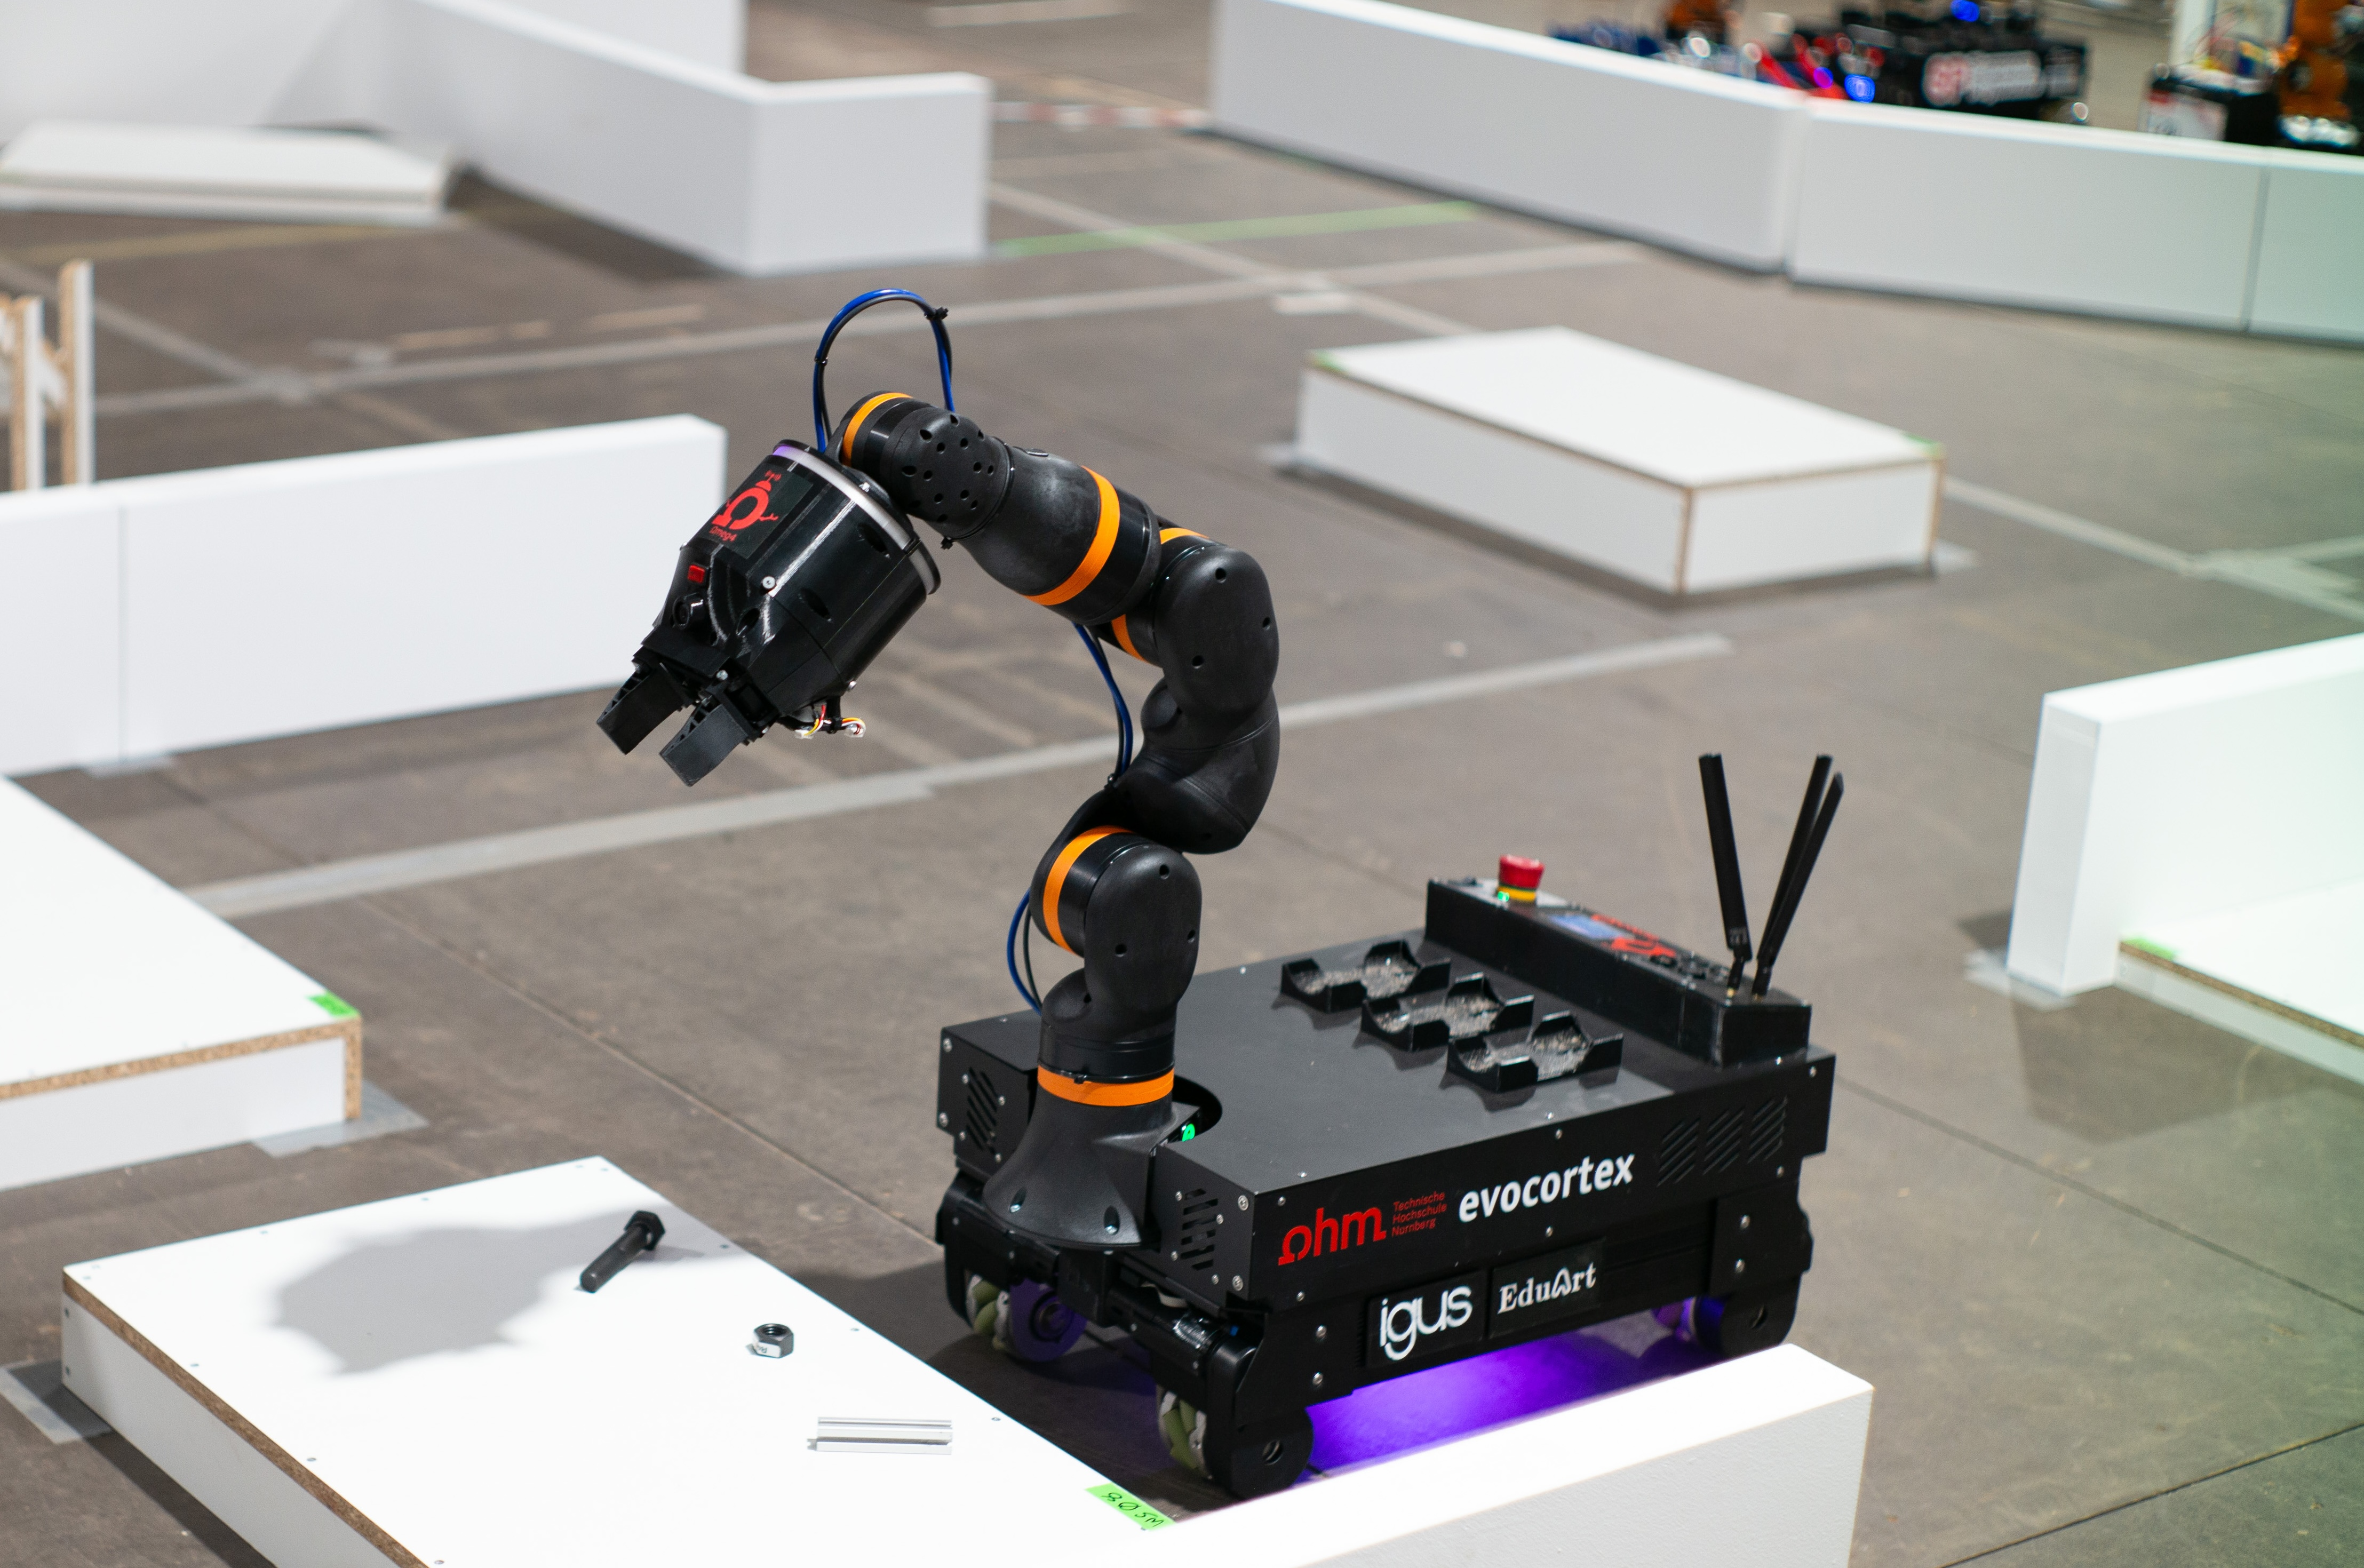
\includegraphics[height=4cm]{img/atwork.jpg}
\end{figure} 


Das Team \textbf{AutonOhm} des Labors für Mobile Robotik nimmt seit vielen Jahren erfolgreich am RoboCup Industrial @Work Wettbewerb teil. Ziel dieses Wettbewerbs ist es, einen mobilen Roboter zu entwickeln, der sich selbstständig in einer Arena zurechtfindet und vordefinierte Aufgaben der Form "Transportiere Gegenstand A von Tisch B zu Tisch C" durchführt. Für diese Aufgaben ist ein komplexes Gesamtsystem aus \emph{Lokalisierung}, \emph{Wahrnehmung}, \emph{Planung} und \emph{Steuerung} notwendig. Es bietet daher für interessierte Studierende neben einer Vielzahl von spannenden Themen im Bereich der mobilen Robotik auch die Möglichkeit, praxisnah an einem \emph{echten} Robotersystem zu arbeiten.

Ziel der Arbeit ist es, eine ROS-Softwarekomponente für die Ansteuerung und Kontrolle des Roboterarms des mobilen Roboters zu entwickeln. Diese Softwarekomponente bekommt von einer Kontrollkomponente im System Kommandos zugesendet, wie z.B. 'Greife Objekt A' oder 'Lege Objekt B aus dem Inventar ab'. Die Komponente muss diese groben Kommandos nun durch eine sinnvolle Koordination und Ablaufsteuerung der involvierten  Systemkomponenten (z.B. Roboterarm, Greifer, Suchlicht etc.) abarbeiten, wobei auch Fehlerzustände und Probleme im Ablauf (z.B. das Verlieren von Objekten) zu berücksichtigen sind.

Die Softwarekomponente soll in das bestehende Gesamtsystem integriert und getestet werden. Engagement und Mitarbeit im studentischen Team AutonOhm sind ausdrücklich erwünscht! Es besteht die Möglichkeit, im Rahmen der Arbeit an nationalen und internationalen Wettbewerben teilzunehmen.

\section*{Arbeitspakete}
\begin{itemize}[leftmargin=0.5cm]
    \setlength\itemsep{.1em}
    \item Einarbeiten in die aktuelle Systemarchitektur des @Work Roboters
    \item Entwicklung einer geeigneten Softwarearchitektur für die Armsteuerung
    \item Implementierung und Validierung der Softwarekomponente in einer Simulationsumgebung 
    \item Integration und Demonstration auf dem Robotersystem 
\end{itemize}

\section*{Voraussetzungen}
\begin{itemize}[leftmargin=0.5cm]
    \setlength\itemsep{.1em}
    \item Grundkenntnisse in einer höheren Programmiersprache (z.B. Python, C++)
    \item Grundkenntnisse in ROS
\end{itemize}

\vspace{0.5cm}
Das Thema kann nach Abstimmung als Bachelor- oder Masterarbeit bearbeitet werden, sowie als Projektarbeit. 


\vfill
\textcolor{ohm_red}{\rule{\linewidth}{0.4mm}}
\textbf{\textcolor{ohm_red}{Labor für mobile Robotik}} \\
\begin{tabular}{@{}ll}
\textbf{Betreuer:} & Prof. Dr. Enrico Schröder \\
\textbf{E-Mail:}   & \href{mailto:enrico.schroeder@th-nuernberg.de}{enrico.schroeder@th-nuernberg.de} \\
\end{tabular}

\end{document}